\documentclass[tikz,border=5pt]{standalone}
\usepackage{amsmath,amssymb}
\begin{document}
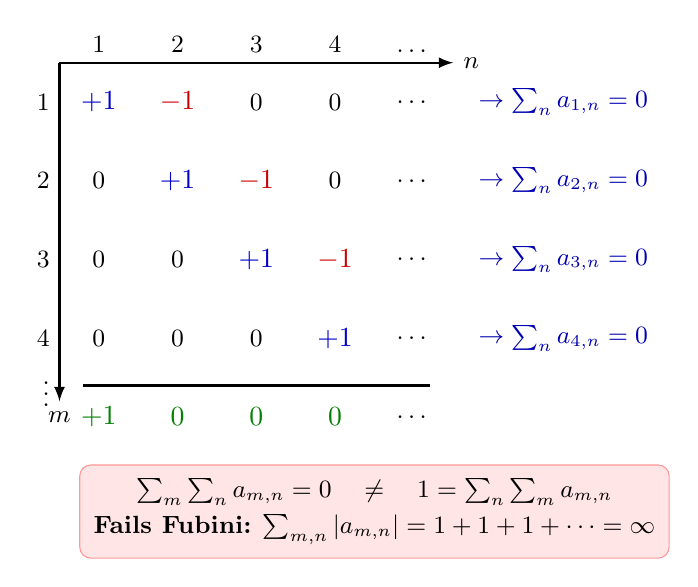
\begin{tikzpicture}[>=latex, font=\small]
  % Grid
  \draw[->, thick] (0.5, 4.5) -- (5.5, 4.5) node[right] {$n$};
  \draw[->, thick] (0.5, 4.5) -- (0.5, 0.2) node[below] {$m$};

  % Coordinates
  \foreach \n in {1, 2, 3, 4} {
    \node[above] at (\n, 4.5) {$\n$};
  }
  \node[above] at (5, 4.5) {$\dots$};

  \foreach \m in {1, 2, 3, 4} {
    \node[left] at (0.5, 5 - \m) {$\m$};
  }
  \node[left] at (0.5, 0.4) {$\vdots$};

  % Matrix values
  % Row 1
  \node[font=\bfseries, text=blue!80!black] at (1, 4) {$+1$};
  \node[font=\bfseries, text=red!80!black] at (2, 4) {$-1$};
  \node at (3, 4) {$0$};
  \node at (4, 4) {$0$};
  \node at (5, 4) {$\dots$};
  \node[anchor=west, color=blue!70!black] at (5.7, 4) {$\to \sum_n a_{1,n} = 0$};

  % Row 2
  \node at (1, 3) {$0$};
  \node[font=\bfseries, text=blue!80!black] at (2, 3) {$+1$};
  \node[font=\bfseries, text=red!80!black] at (3, 3) {$-1$};
  \node at (4, 3) {$0$};
  \node at (5, 3) {$\dots$};
  \node[anchor=west, color=blue!70!black] at (5.7, 3) {$\to \sum_n a_{2,n} = 0$};

  % Row 3
  \node at (1, 2) {$0$};
  \node at (2, 2) {$0$};
  \node[font=\bfseries, text=blue!80!black] at (3, 2) {$+1$};
  \node[font=\bfseries, text=red!80!black] at (4, 2) {$-1$};
  \node at (5, 2) {$\dots$};
  \node[anchor=west, color=blue!70!black] at (5.7, 2) {$\to \sum_n a_{3,n} = 0$};

  % Row 4
  \node at (1, 1) {$0$};
  \node at (2, 1) {$0$};
  \node at (3, 1) {$0$};
  \node[font=\bfseries, text=blue!80!black] at (4, 1) {$+1$};
  \node at (5, 1) {$\dots$};
  \node[anchor=west, color=blue!70!black] at (5.7, 1) {$\to \sum_n a_{4,n} = 0$};

  % Column sums
  \draw[thick] (0.8, 0.4) -- (5.2, 0.4);
  \node[font=\bfseries, text=green!50!black] at (1, -0.0) {$+1$};
  \node[font=\bfseries, text=green!50!black] at (2, -0.0) {$0$};
  \node[font=\bfseries, text=green!50!black] at (3, -0.0) {$0$};
  \node[font=\bfseries, text=green!50!black] at (4, -0.0) {$0$};
  \node at (5, -0.0) {$\dots$};

  % Summary
  \node[align=center, fill=red!10, draw=red!40, rounded corners, inner sep=5pt] at (4.5, -1.2)
    {$\sum_m \sum_n a_{m,n} = 0 \quad\neq\quad 1 = \sum_n \sum_m a_{m,n}$ \\[2pt]
     \textbf{Fails Fubini:} $\sum_{m,n} |a_{m,n}| = 1 + 1 + 1 + \dots = \infty$};
\end{tikzpicture}
\end{document}
